\section{Introduction}
\label{sec:intro}

%In recent years, the barriers to the development of Artificial Intelligence (AI) have been broken down with the rapid progress of ABC technologies in computing: AI, Big Data, and Cloud Computing, as well as the emergence of cost-effective specialized hardware~\cite{sze2017efficient} and software~\cite{jia2014caffe}. This has led to the world entering the third wave of AI development: Deep Learning~\cite{lecun2015deep}.
The success of current data-driven AI relies on massive amounts of training data and follows a gather-and-analyze paradigm~\cite{whang2023data}, which confronts with challenges of complying with rigorous data protection regulations such as OECD Privacy Guidelines~\cite{tene2011privacy} and GDPR~\cite{voigt2017eu}.
%Although data-centric AI is now the mainstream, a novel model-centric distributed collaborative training framework called Federated Learning is gaining popularity in both academia and industry due to its advantages in complying with privacy regulations.
Although data-centric AI is currently mainstream paradigm, Federated Learning~\cite{li2020federated}, a novel distributed collaborative training framework, is gaining popularity in both academia and industry for its advantages in complying with privacy regulations~\cite{truong2021privacy}.

%According to the definitions of IEEE Standard for Federated Machine Learning (FML, aka FL)~\cite{IEEEstd3652}, \textit{FL is a framework or system that enables multiple participants to collaboratively build and use machine learning models without disclosing the raw and private data owned by the participants while achieving good performance.}
%For example, a typical workflow of FL systems is that the entity with modeling demand (FL server) first deploys the FL services and initializes the training task, and then distributes this task to participants with training data (FL clients) for modeling~\cite{bonawitz2019towards}.
A typical workflow of FL systems is presented in Fig.\ref{fig:coop}(a), where the entity with a modeling demand (FL server) first deploys the FL services, initializes the training task, and then distributes this task to participants with training data (FL clients) for modeling\cite{bonawitz2019towards}.
Based on this workflow pattern, FL frameworks have been derived with specialized improvements in communication~\cite{konevcny2016federated, mcmahan2017communication, xu2023asynchronous}, optimizaiton~\cite{li2018federated, karimireddy2020scaffold, li2021model}, robustness~\cite{duan2020self, sattler2019robust, li2022federated} and privacy~\cite{bonawitz2017practical, geyer2017differentially, cheng2021secureboost}.
While these fascinating improvements greatly enhance the utility of FL, they all follow a task-based interaction paradigm, in which an FL server dominates the cooperation.
In this narrow interpretation of FL, the data owner is treated more like a worker than a collaborator and performs training primarily for the benefit of the server's goals.
Due to the above defects, FL clients have little enthusiasm to participate, and the potential for redundant training also leads to low model reusability, further diminishing the efficiency of the FL systems.
%This explains why current FL frameworks are more akin to private distributed modeling services rather than sustainable and privacy-preserving modeling platforms for everyone as expected.
This explains why current FL frameworks are more akin to private distributed modeling services rather than open and sustainable modeling platforms that every user can access and benefit from, addressing many data silo applications.

\begin{figure*}[tbh]
    \centering
    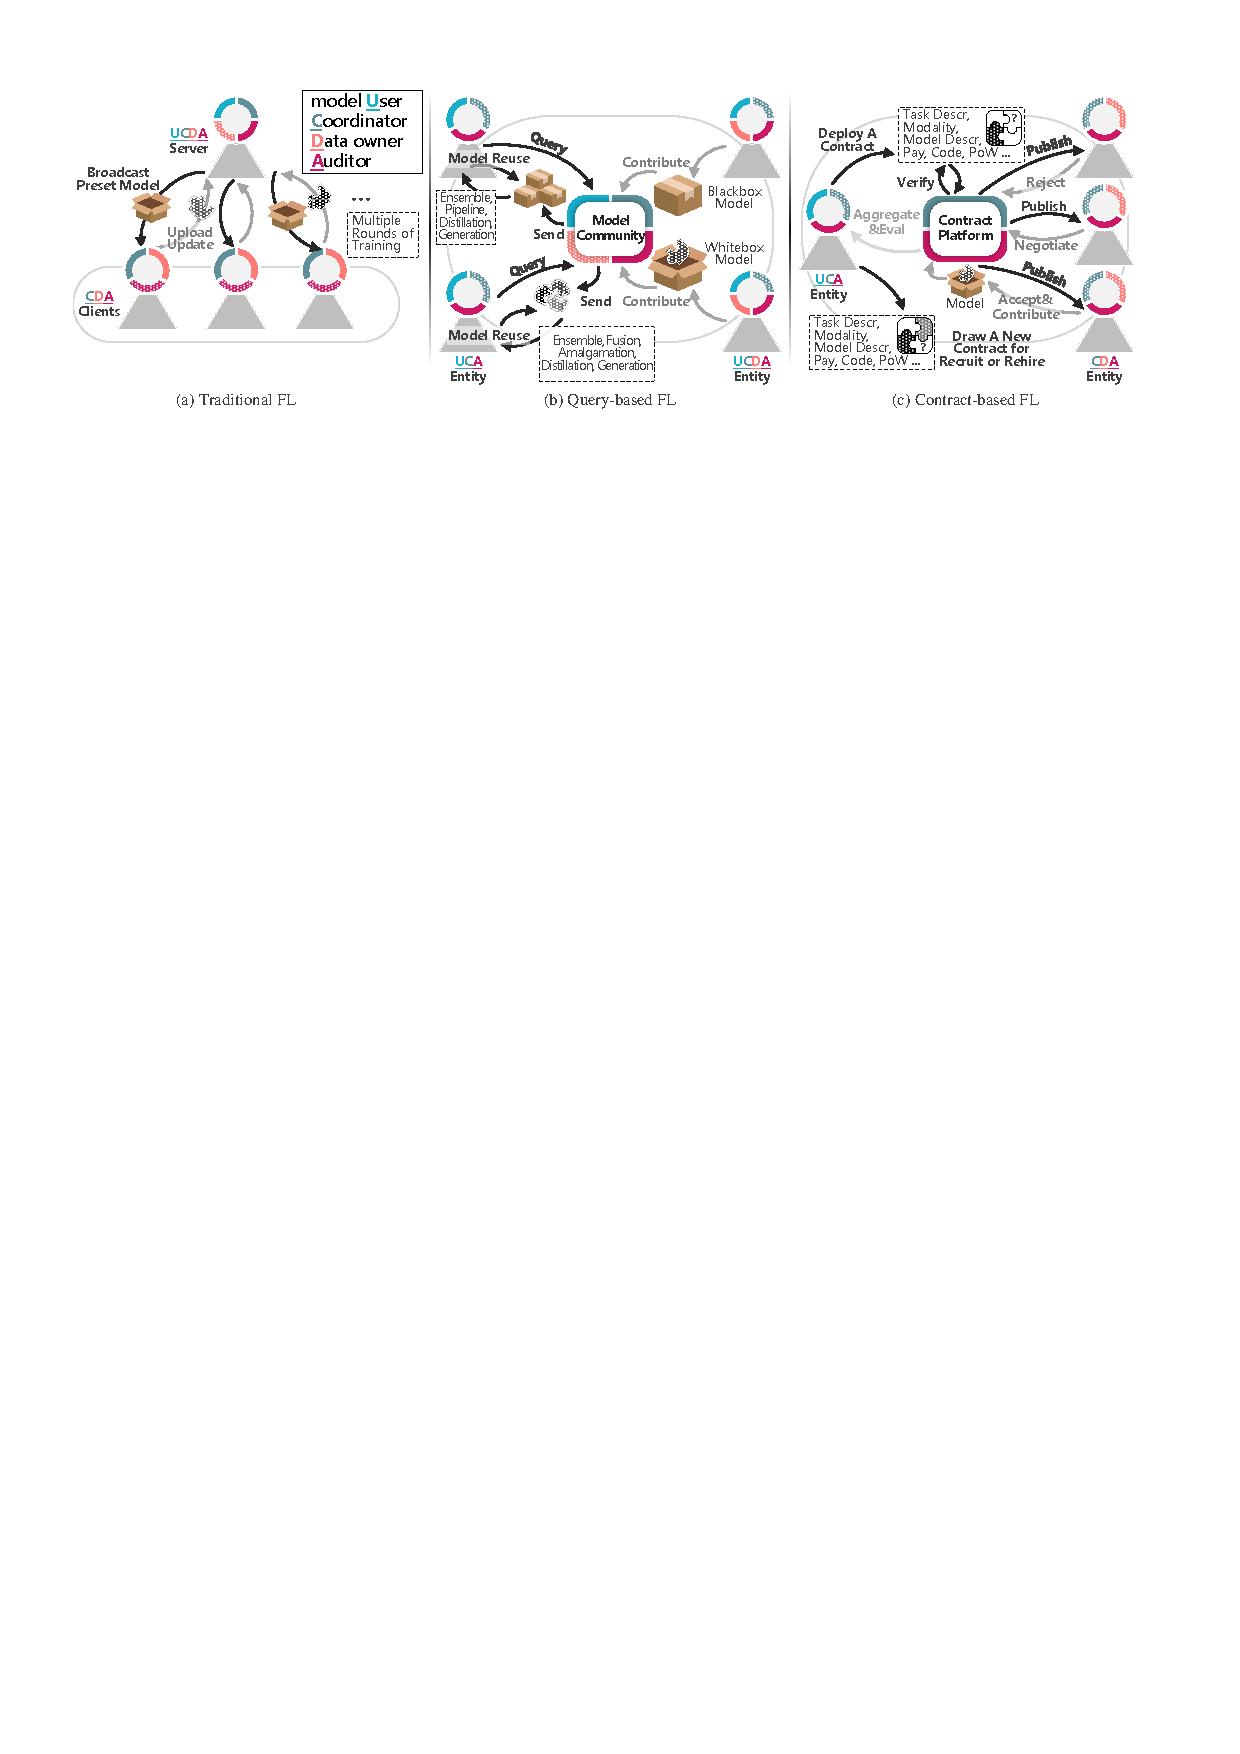
\includegraphics[scale=0.9]{fig/coop_frame.pdf} % width=\linewidth
    \caption{A schematic diagram of three cooperation frameworks of FL. (a) is the traditional FL platform, (b)~(c) are the proposed open FL platforms. Four colors correspond to four roles in~\cite{IEEEstd3652}, and colors with grid lines indicate non-essential roles.}
    \label{fig:coop}
\end{figure*}

In this paper, we try to answer the question: \textbf{Can we establish a sustainable open FL platform based on a novel reciprocal cooperation framework?}
Obviously, to answer this quesion, it is insufficient to simply study the basic concepts of FL and investigate existing FL techniques.
We also need to conduct a wide survey of potential techniques that can facilitate the construction of open FL platforms.
To aid understanding, Fig.~\ref{fig:coop}(b)(c) provide a first glimpse of two novel FL cooperation frameworks that we advocated: 
\begin{itemize}
    \item \textbf{Query-based FL}. It follows a loosely-coupled cooperation framework between entities (we use "entities" instead of "clients" to emphasizes equality), where any entity can freely upload their local models or query models from an open repository named \textit{Model Community}.
    There are many valuable challenges that can be explored, such as how to query for models, how to reuse the retrieved models or how to transfer knowledge from these models, how to ensure the legal compliance between different model licenses, and how to protect the intelligent properties of released models (ref. \S\ref{sec:query}, \S\ref{sec:taxonomy} and \ddag{II}, \ddag{III}, \ddag{IV}, \ddag{V}, where \S~denotes the main section and \ddag~denotes the appendix section). %TODO: 
    \item \textbf{Contract-based FL}. It follows a mutual choice cooperation framework, where each entity can deploy model training contracts with specialized requirements such as task modality, execution environment, model architecture and license. Meanwhile, entities holding data can choose whether to accept the contract.
    We show the research topics in this setting include ML subtasks design and monetization (ref. \S\ref{sec:contract} and \ddag{VI}).
    %model pricing, model contribution evaluation and so on.% and .... (ref. Section~\ref{}) % TODO:
\end{itemize}
It is worth noting that the definitions of the four roles illustrated in Fig.~\ref{fig:coop} (i.e., model user, coordinator, data owner, auditor, ref. \S\ref{sec:basicdefinition}) are adopted for compatibility with the IEEE standard~\cite{IEEEstd3652}, and our proposals are also within the standard definitions of FL.
The diagram in Fig.~\ref{fig:coop}(a) illustrates the workflow of traditional FL, where all FL clients are required to accept the training schedule from the FL server and perform multiple rounds of local training and model averaging until the global model converges.
In contrast, the entities in query-based FL and contract-based FL are proactive in their participation.
We believe that these reciprocal cooperation frameworks have the potential to expand the prevalence of open FL and establish FL ecosystems.


\subsection{Our Contribution}
\label{sec:contribution}
  In contrast to previous surveys that primarily focused on the server-dominated cooperation framework in FL (ref. \S\ref{sec:related}),  our new survey explores the feasibility of reciprocal cooperation frameworks in FL.
  To the best of our knowledge, our work represents the first systematic survey in this area.
  The major contributions of this survey are as follows:
  \begin{itemize}
      \item We are the first to introduce the concept of open FL platforms by presenting two cooperation frameworks, namely query-based FL and contract-based FL, along with an overview of their key features and properties.
      \item We explore the query functionalities of online model repositories, such as Huggingface and OpenVINO, to investigate their feasibility for model query in query-based FL settings.
      \item We summarize the rights, restrictions, and enforcements of in-service model licenses and highlight the legal compliance and copyrightability issues in collaborative modeling. Additionally, we provide guidelines for selecting licenses to minimize conflicts and prevent license proliferation.
      \item We propose a taxonomy to streamline the legal compliance analysis in ML, which is also useful for quickly identifying suitable model reusing conceptss for open FL platforms. A comprehensive comparison of current FL studies based on this taxonomy is surveyed.
      \item We analyze the requirements for model protection in the context of query-based FL and identify applicable solutions from deep Intellectual Property (IP) protection. We also introduce the concept of designing ML microtasks for query-based FL.
\end{itemize}

\begin{comment}
The rest of this paper is organized as follows. 
We compare this survey to other related surveys and show our distinction in Section~\ref{sec:related} and Appendix~I. 
In Section~\ref{sec:basic}, we present the overview and point the limitations of traditional FL.
We comprehensively explore the feasibility and challenges of query-based FL in Section~\ref{sec:query}, which includes model query (Section~\ref{sec:how2query} and Appendix~II), model license comparison (Section~\ref{sec:licensing}) and license selection (Section~\ref{sec:choosing} and Appendix~III), copyright issues (Appendix~III.D), and analysis of license conflicts in model reusing (Appendix IV.B).
In Section~\ref{sec:taxonomy}, we present our taxonomy from a model reusing perspective, and in Appendix IV.A, we summarize FL studies based on this new taxonomy.
The discussion on model IP protection is presented in Appendix V.
We introduce how to design ML microtasks in contract-based FL in Section~\ref{sec:contract}, and we leave the discussion about decentralization and monetization to Appendix~VI.
\end{comment}

The structure of this paper is shown in Fig.~\ref{fig:article_structure}. 
We compare this survey to other related surveys and show our distinction in \S\ref{sec:related}. 
In \S\ref{sec:basic}, we present the overview and point the limitations of traditional FL.
We comprehensively explore the feasibility and challenges of query-based FL in \S\ref{sec:query}, which includes model query (\S\ref{sec:how2query}), model license comparison (\S\ref{sec:licensing}) and license selection (\S\ref{sec:choosing}).
In \S\ref{sec:taxonomy}, we present our taxonomy from a model reusing perspective.
We introduce how to design ML microtasks in contract-based FL in \S\ref{sec:contract} and we conclude this paper in \S\ref{sec:conclusion}.
\emph{Due to page limits, we defer some related discussions to the appendix and we use \ddag{} to remind you that detailed analysis can be found in the appendix.}

\begin{figure}[h]
    \centering
    \label{fig:article}
    \resizebox{\columnwidth}{!}{
      \begin{tikzpicture}[
        >=stealth,
        node distance=0.6cm,
        thick,
        main node/.style={rectangle, draw, fill=Employer!30, text width=2.1cm, text centered, rounded corners, minimum height=0.6cm, font=\small},
        sub node/.style={rectangle, draw, fill=Worker!30, text width=1.5cm, text centered, rounded corners, minimum height=0.5cm, font=\footnotesize},
        apdx node/.style={rectangle, draw, fill=Platform!30, text width=1.5cm, text centered, rounded corners, minimum height=0.5cm, font=\footnotesize},
        every edge/.style={draw, thick, ->}
      ]
      % Nodes
      \node[main node] (intro) {\fullref{sec:intro}};
      \node[main node, right=of intro] (related) {\fullref{sec:related}};
      \node[main node, right=of related] (concepts) {\hyperref[sec:basic]{\S\textbf{\ref{sec:basic}}. Basic FL Concepts}};
      \node[main node, right=of concepts] (qbfl) {\hyperref[sec:query]{\S\textbf{\ref{sec:query}}. Query-based FL}};
      \node[main node, right=of qbfl] (elli) {\textbf{\dots}};
      \node[main node, below=3cm of intro] (reuse) {\fullref{sec:taxonomy}};
      \node[main node, right=2cm of reuse] (remain) {\hyperref[sec:remaining_qbfl]{\S\textbf{\ref{sec:remaining_qbfl}}. Remaining Topics}};
      \node[main node, below=4cm of qbfl] (cbfl) {\hyperref[sec:contract]{\S\textbf{\ref{sec:contract}}. Contract-based FL}};
      \node[main node, right=0.6cm of cbfl] (conclusion) {\fullref{sec:conclusion}};
      
     % Arrows
     \path (intro) edge (related);
     \path (related) edge (concepts);
     \path (concepts) edge (qbfl);
     \path (qbfl) edge (elli);
     \path (reuse) edge (remain);
     \path (remain) edge (cbfl);
     \path (cbfl) edge (conclusion);
        
      % Subnodes
      % Introduction
      \node[below=0.4cm of intro, sub node] (intro_sub1) {\fullref{sec:contribution}};
      \draw[->] ([xshift=-0.5cm] intro.south) -- ++(0.15,-0.15) -|  (intro_sub1.north);

      % Related Surveys
      \node[below=0.4cm of related, apdx node] (related_sub1) {\ddag{I}. Related Topics};
      \node[below left=0.3cm and -0.8cm of related_sub1, apdx node] (related_sub2) {As-a-Service};
      \node[below right=0.3cm and -0.8cm of related_sub1, apdx node] (related_sub3) {Dcentralized FL};
      \node[below left=0.3cm and 1.1cm of related_sub1, apdx node] (related_sub4) {FL Systems};
      \draw[->] ([xshift=-0.5cm] related.south) -- ++(0.15,-0.15) -|  (related_sub1.north);
      \draw[->] (related_sub1) -- (related_sub2);
      \draw[->] (related_sub1) -- (related_sub3);
      \draw[->] (related_sub1) -- (related_sub4);
      
      % Basic Concepts of FL
      \node[below=0.4cm of concepts, sub node] (concepts_sub1) {\fullref{sec:basicdefinition}};
      \node[below=0.3cm of concepts_sub1, sub node] (concepts_sub2) {\hyperref[sec:limitations_FL]{\S\textbf{\ref{sec:limitations_FL}}. Limitations of FL}};
      \draw[->] ([xshift=-0.5cm] concepts.south) -- ++(0.15,-0.15) -|  (concepts_sub1.north);
      \draw[->] (concepts_sub1) -- (concepts_sub2);

      % Query-based FL
      \node[below=0.4cm of qbfl, sub node] (qbfl_sub1) {\fullref{sec:query_overview}};
      \node[below left=0.3cm and -0.8cm of qbfl_sub1, sub node] (qbfl_sub2) {\hyperref[sec:how2query]{\S\textbf{\ref{sec:how2query}}. How to Query}};
      \node[below left=0.3cm and -1.5cm of qbfl_sub2, sub node] (qbfl_sub3) {\hyperref[sec:how2reuse]{\S\textbf{\ref{sec:how2reuse}}. Legal Issues}};
      \node[right=0.2cm of qbfl_sub2, apdx node] (qbfl_sub4) {\ddag{II}. Filter Conditions};
      \node[below=0.4cm of qbfl_sub4, apdx node] (qbfl_sub5) {\ddag{III}. License Choosing};
      \node[right=0.3cm of qbfl_sub5, apdx node] (qbfl_sub6) {Copy-rightability};
      \node[above=0.3cm of qbfl_sub6, apdx node] (qbfl_sub7) {Datasets, Software, Models Licenses};
      \draw[->] ([xshift=-0.5cm] qbfl.south) -- ++(0.15,-0.15) -|  (qbfl_sub1.north);
      \draw[->] (qbfl_sub1) -- (qbfl_sub2);
      \draw[->] (qbfl_sub2) -- (qbfl_sub3);
      \draw[->] (qbfl_sub2) -- (qbfl_sub4);
      \draw[->] (qbfl_sub3) -- (qbfl_sub5);
      \draw[->] (qbfl_sub5) -- (qbfl_sub6);
      \draw[->] (qbfl_sub5) -- (qbfl_sub7);

      % Batch Model Reuse Mechanisms
      \node[below=0.4cm of reuse, sub node] (reuse_sub1) {\hyperref[sec:combination]{Combination}, \hyperref[sec:amalgamation]{Amalgam...}, \hyperref[sec:distillation]{Distillation}, \hyperref[sec:generation]{Generation}};
      \node[below=0.4cm of reuse_sub1, sub node] (reuse_sub2) {\hyperref[sec:how2query]{\S\textbf{\ref{sec:how2query}}. Hybrid Model Reusing...}};
      \node[right=0.3cm of reuse_sub2, apdx node] (reuse_sub3) {\ddag{IV-B}. Model Reusing vs. Model Licenses};
      \node[above=0.2cm of reuse_sub3, apdx node] (reuse_sub4) {\ddag{IV-A}. Hybrid Model Reusing in FL};
      \draw[->] ([xshift=-0.5cm] reuse.south) -- ++(0.15,-0.15) -|  (reuse_sub1.north);
      \draw[->] (reuse_sub1) -- (reuse_sub2);
      \draw[->] (reuse_sub2) -- (reuse_sub3);
      \draw[->] (reuse_sub2) -- (reuse_sub4);

      % Remaining Topics
      \node[below=0.4cm of remain, sub node] (remain_sub1) {\fullref{sec:ip_protect}};
      \node[below=0.4cm of remain_sub1, sub node] (remain_sub2) {\fullref{sec:limitations_qbfl}};
      \node[right=0.3cm of remain_sub1, apdx node] (remain_sub3) {\ddag{V}. How to Protect Models};
      \draw[->] ([xshift=-0.5cm] remain.south) -- ++(0.15,-0.15) -|  (remain_sub1.north);
      \draw[->] (remain_sub1) -- (remain_sub2);
      \draw[->] (remain_sub1) -- (remain_sub3);

      \node[below=0.4cm of cbfl, sub node] (cbfl_sub1) {\fullref{sec:contract_overview}};
      \node[below right=-0.8cm and 1.3cm of cbfl_sub1, apdx node] (cbfl_sub2) {\ddag{VI}. Decentralization and Monetization in Contract-based FL};
      \node[below left=0.4cm and -0.7cm of cbfl_sub1, sub node] (cbfl_sub3) {\fullref{sec:how2design}};
      \node[below right=0.4cm and -0.7cm of cbfl_sub1, sub node] (cbfl_sub4) {\fullref{sec:limitations_cbfl}};
      \draw[->] ([xshift=-0.5cm] cbfl.south) -- ++(0.15,-0.15) -|  (cbfl_sub1.north);
      \draw[->] (cbfl_sub1) -- (cbfl_sub2);
      \draw[->] (cbfl_sub1) -- (cbfl_sub3);
      \draw[->] (cbfl_sub3) -- (cbfl_sub4);
      

      \begin{scope}[on background layer]
        \draw[->, dashed, line width=1pt, dash pattern=on 2pt off 2pt, draw=Employer, opacity=0.7] (elli.south) -- (reuse.north);
      \end{scope}

      \end{tikzpicture}
    }
    \caption{Article Structure. \S: \colorbox{Employer!30}{Main Section}\colorbox{Worker!30}{Subsection}, \ddag: \colorbox{Platform!30}{Appendix}.}
    %\caption{Article Structure. \S: \textcolor{Employer!30}{Main Text Section}, \ddag: \textcolor{Platform!30}{Appendix Section}.}
    \label{fig:article_structure}
\end{figure}


%license selection (Section~\ref{sec:choosing} and Appendix~III), copyright issues (Appendix~III.D), and analysis of license conflicts in model reusing (Appendix IV.B).
%In Section~\ref{sec:taxonomy}, we present our taxonomy from a model reusing perspective, and in Appendix IV.A, we summarize FL studies based on this new taxonomy.
%The discussion on model IP protection is presented in Appendix V.
%We introduce how to design ML microtasks in contract-based FL in Section~\ref{sec:contract}, and we leave the discussion about decentralization and monetization to Appendix~VI.

%We conclude the paper in Section VII.

%By investigating reciprocal cooperation frameworks, we aim to broaden the understanding of FL and uncover new opportunities for collaboration and data sharing among participants. Through our comprehensive analysis, we provide valuable insights and recommendations for researchers and practitioners interested in exploring and implementing reciprocal cooperation in FL settings.
